\chapter{Expermental Setup}
\label{chapter-5}

\section{Proposed Setup}

This section describes the proposed setup for motion tracking suit and humanoid robot, NAO. Figure \ref{fig: experimental-setup} represents the environment setup for this research.
The first stage of this research was to implement the motion imitation with ZMP balance control. This implementation helps the initial validation of the capabilities for real-time motion imitaion, 
as well as processing the human data. In this case, the single support is initially tested since NAO robot will never lose it's balance when moving it's hands.

\begin{figure}[h!]
    \centering
    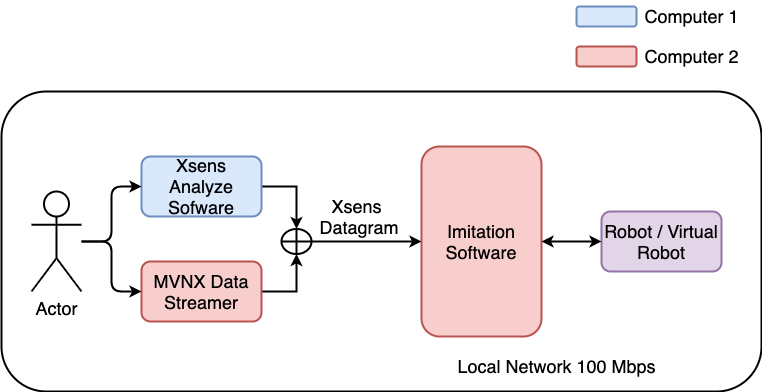
\includegraphics[scale=0.5]{images/flowchart-experimental-setup.png}\hfill
    \caption{Illustration of the experimental setup}\hfill
    \label{fig: experimental-setup}
\end{figure}

\section{NAO robot platform}


NAO is a programmable, autonomous, 57 cm tall humanoid robot developed by Aldebaran Robotics, a French startup company. The biped is equipped with several
different sensors, including an inertial measurement unit with accelerometer, gyrometer and four ultrasonic sensors that provide NAO with stability and 
positioning within space, in addition eight force-sensing resistors and two bumpers. It features an Intel ATOM 1,6 GHz CPU, located in the head, that runs
 a Linux kernel and a second CPU located in the torso.


\begin{figure}[h!]
    \centering
    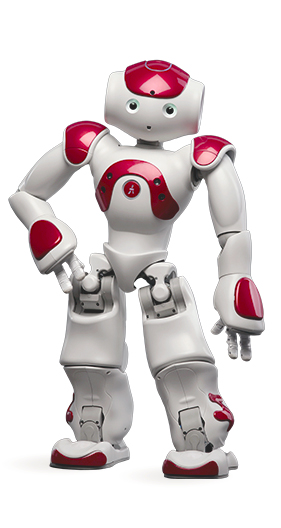
\includegraphics[scale=0.55]{images/nao-robot.jpg}\hfill
    \caption{NAO - Aldebaran Robotics \cite{aldebaran-masses}}\hfill
    \label{fig: nao-robot}
\end{figure}

NAO has a total of 25 degrees of freedom (DOF), 11 DOF for the lower part that includes legs and pelvis, and 14 DOF for the upper part that includes trunk, 
arms and head. Each leg has 2 DOF at the ankle, 1 DOF at the knee and 2 DOF at the hip. A special mechanism composed of two coupled joints at each hip equips 
the pelvis. The rotation axis of these two joints are inclined at $45^\circ$ towards the body. This mechanism replaces the classical set of three active rotary joints 
encountered in most humanoid robots.


Aldebaran Robotics provides a complete documentation for the robot, based on a geometric model shown in their website \cite{aldebaran-masses}. The model of the lower body of the robot 
NAO is obtained considering the two legs identical and identically actuated. The two revolute joints that constitute the pelvis and named separately, but 
they essentially represent a unique actuated DOF. To conclude, it is important to remark that, unlike prototypes such as Wabian-2R or LOLA, the foot sole of 
the present version of NAO does not feature any passive or active joint that would enhance higher speed gait performances.


\subsection{NAOqi C++ SDK}

The robot's embedded software, \textit{NAOqi}, a framework so the robot can be programmed in various operating systems, and in various languages, including C++, Python and MATLAB. 
The manufacturer also provides a software, \textit{choreographe} allows connecting to the real robot through local network and starts the NAOqi service in the robot.
\textit{Choreographe} can also be used as a graphical interface for block-programming to interact with the robot.

In this research, the software is developed in C++ for interaction with the real robot and compiled with CMake, a cross compiled platform for build systems, to make use of 
NAOqi libraries. The support for NAO v5 humanoid framework is provided in NAOqi version 2.1.4 and is used for both real robot and simulation. The NAOqi 2.1.4 applications could be build in unix-systems by custom cross-compiler \textit{qibuild}, a cmake extension and a python 2.7 module developed by Aldebaran 
Robotics. At the time of research, python 2.7 is completely abandoned. To make use of the functionalities of \textit{qibuild}, the module is built from source on python 3.8.

The software is developed on unix-system and ran in a seperate windows computer communicating with the robot through local network. The software is developed as a standalone build for suitable version control using \textit{git} and is available in 
\cite{github}.

\subsection{CopelliaSim support}
To simulate the dynamic behaviour during motion retargetting, the work is initially planned to simulate the robot in robotics simulators like Gazebo, Webots and CopelliaSim. 
The support for Webots and Gazebo has been dropped by Aldebaran community at the time of the research. Hence, the existing model of NAO robot in CopelliaSim is used to interact 
with NAOqi services and proxies. 


\begin{figure}[h!]
    \centering
    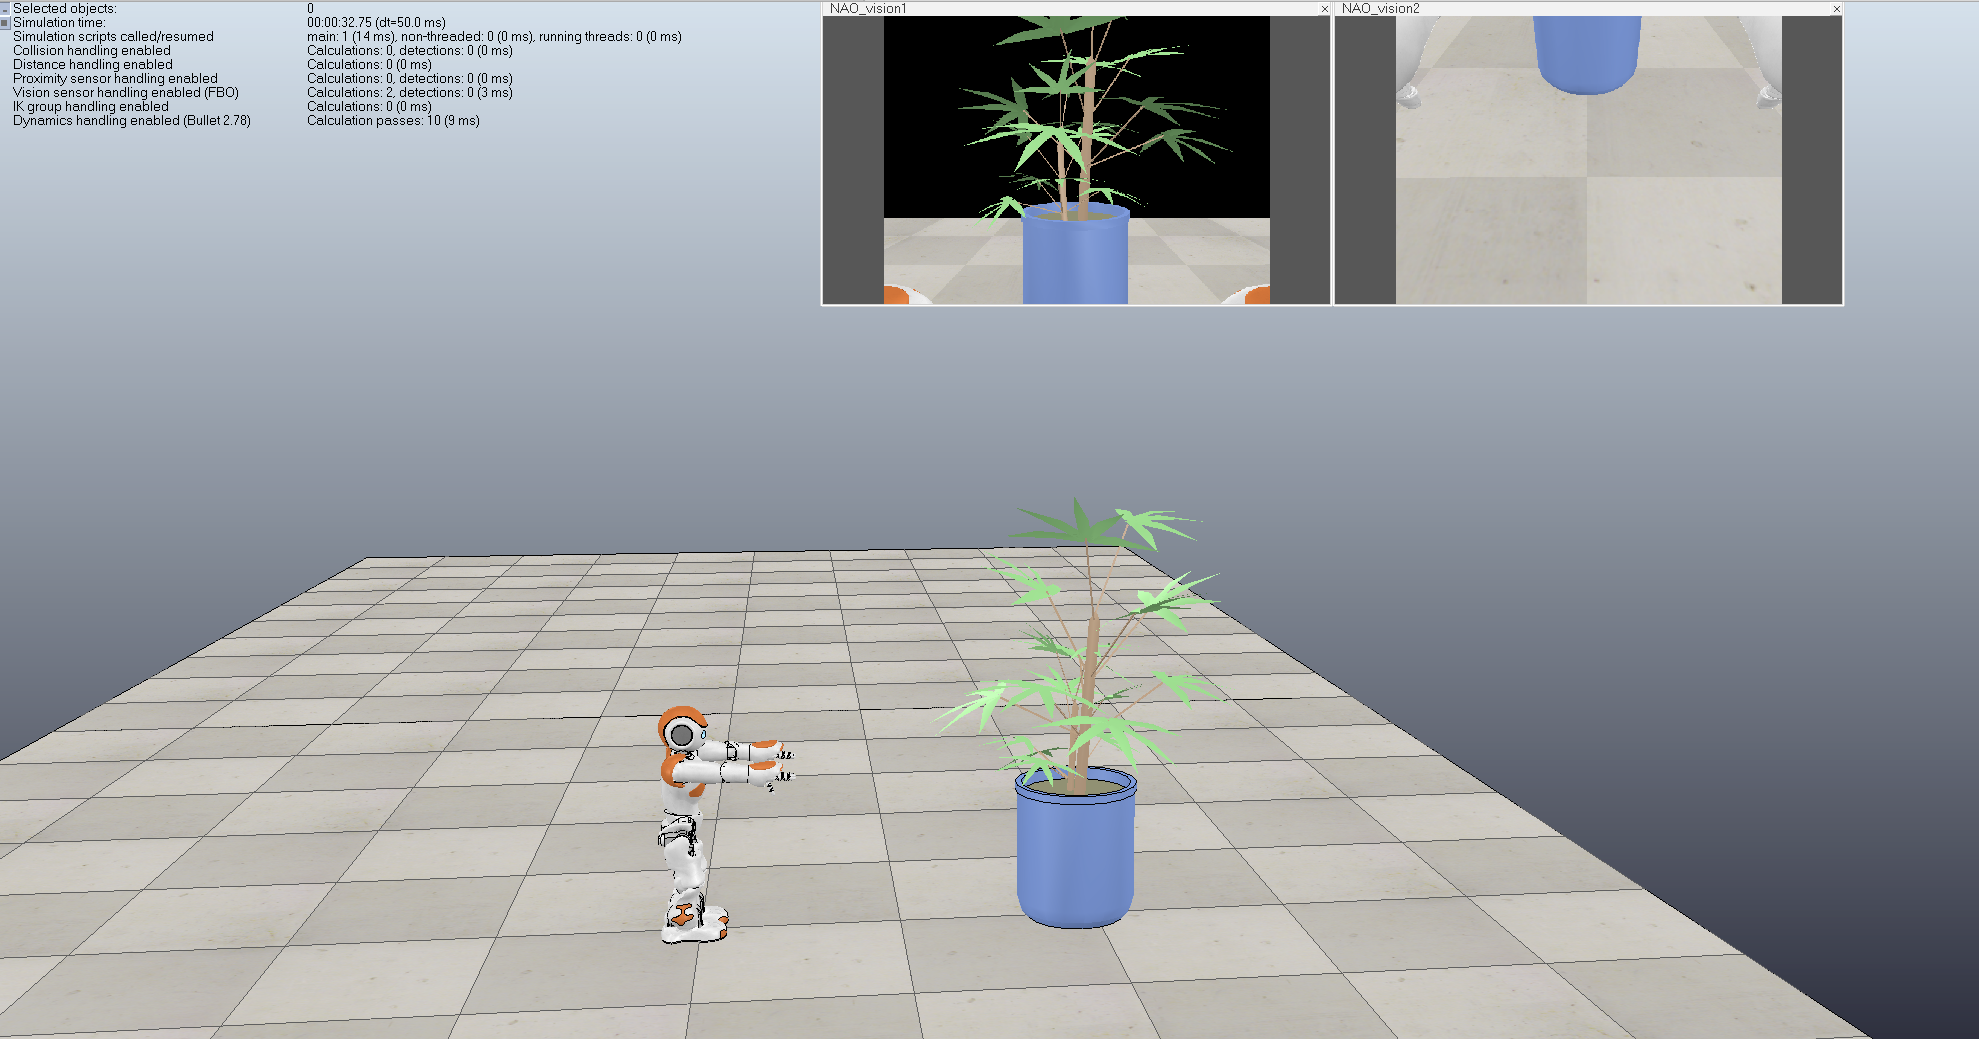
\includegraphics[scale=0.235]{images/copellia-sim.png}\hfill
    \caption{NAO robot in CopelliaSim simulator}\hfill
    \label{fig: copellia-sim}
\end{figure}

Figure \ref{fig: copellia-sim} presents the simulation of NAO robot and the interaction of Visual proxies from NAOqi services. The simulation is 
used as a testing platform to monitor the initial behaviour during the imitation process, although there are evidences that the simulators doesn't replicate exactly the dynamic 
behaviour of the humanoid robot in the real world \cite{ramosponce}. 

\section{Xsens MVN Analyze}

MVN Analyze/Animate, developed by Xsens, is a tool to capture and compute the 6DOF motion data of an inertial sensor-driven system. It allows the export of the data to third party 
applications such as Motion Builder, making the data available to drive rigged characters in e.g. animations. The data transfer to other applications is primarily file based when using MVN Analyze/Animate. With the XME API (SDK) there are many other options.
Typically, Xsens inertial sensor technology is used for orientation, attitude- and positioning data. The technology is integrated by fleet operators, robotics integrator, digital mapping companies, drone developers, Vehicle-testing, Autonomous Vehicles, Warehouse 
and Logistics (AGV/AMR), Maritime/offshore, Aerospace, Heavy-Industry and Agriculture.In robotics research community, the MVN analyze system is used for motion imitation purposes due to its low-cost efficient sensor suit. This section describes the sensor suit setup and 
network streaming protocol over UDP networking.

\begin{figure}[h!]
    \centering
    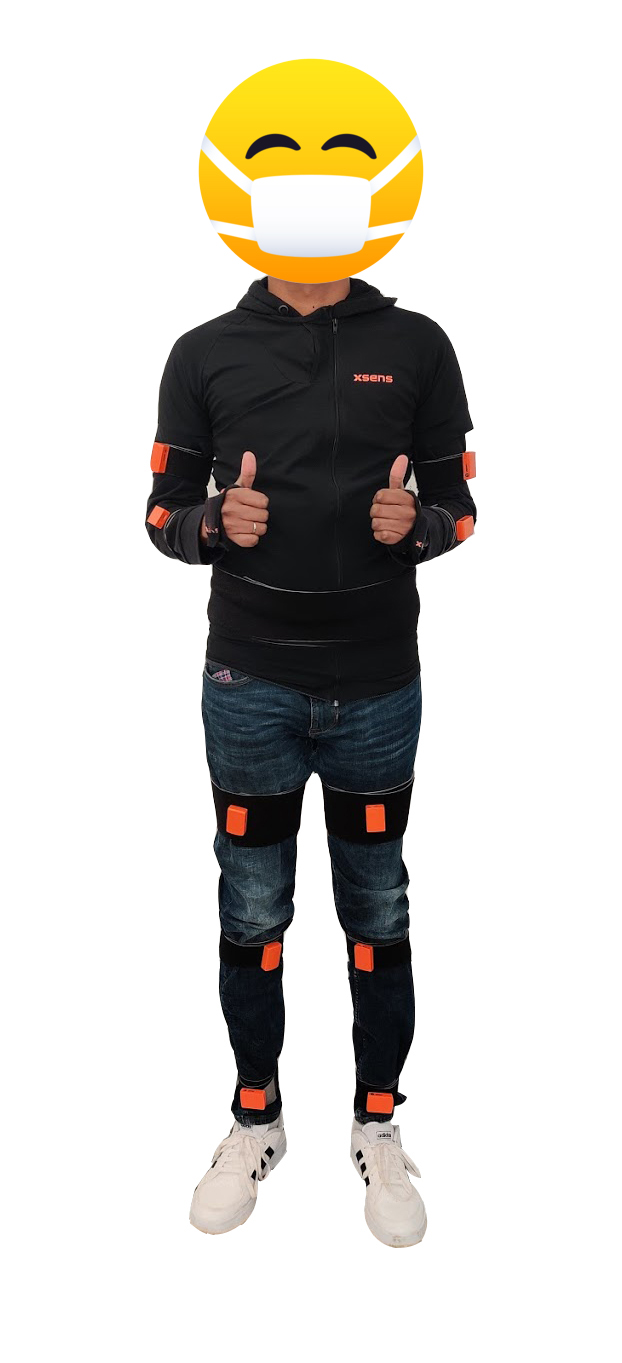
\includegraphics[scale=0.235]{images/xsens-suit.jpg}\hfill
    \caption{Xsens MVN Analyze Suit}\hfill
    \label{fig: xsens-suit}
\end{figure}

\subsection{Sensor Setup}
The hardware of Xsens MVN is available as a body-wired solution that streams data wirelessly to a PC/laptop (MVN Link) and a completely wireless solution(MVN Awinda). 
In the field of humanoid robotics and bio-mechanics, to capture the motion of the human body, 17 motion trackers are attached to the feet, lower legs, upper legs, pelvis, shoulders, sternum, head, upper arms, fore arms, and hands. The sensor modules are inertial and magnetic measurement units that contain 3D gyroscopes, 3D accelerometers and 3D magnetometers.

Each module comes with higher sensor fusion algorithms, with advnced signal processing frameworks like StrapDown Integration (SDI). Due to the use of SDI, 3D tracking accuracy of each motion tracker is equivalent both for MVN Link (240 Hz) as well as MVN Awinda (60 Hz), 
with only a reduced time resolution for the latter. Hence, for high dynamic movements including frequent interactions with the floor (contacts), MVN Link is recommended. Xsens MVN framework provides implementation in C++ and python. The Software Development Kit (SDK) allows 
fetching raw data for direct manipulation to our wishes. It can be noted that the Xsens software has to setup to enable data sharing available outside the software.

\subsection{Xsens Networking Protocol}

The streaming feature in Xsens software enables the computer that run MVN Analyze to stream the captured data over a network to other client computers (in this case, 
the windows computer that runs imitation software). The network environment will be assumed to be a local 100 Mbit Ethernet network, larger network topologies are not 
considered and can be covered by file transfer of the already given file export functionality or later extensions to the network protocol. Thus, few packet loss or data 
corruption during transfer is to be expected, as well as constant connectivity.

Network communication uses a protocol stack, thus the streaming protocol will be implemented on top of a given set of protocols already available for the network clients. 
In this case, the layers to build upon are IP and UDP (or TCP, which is also supported). IP (Internet Protocol, RFC 791) is the network layer protocol used in Ethernet networks 
and defines the source and destination of the packets within the network. Upon this, UDP (User Datagram Protocol, RFC 768) is used to encapsulate the data. The UDP Protocol is 
unidirectional, and contrary to TCP (Transmission Control Protocol, RFC 793) it is stateless and does not require the receiver to answer incoming packets. This allows greater speed.
The default port for xsens network streamer is 9763 and can be changed if needed.

\subsection{Datagram Protocol}

The motion capture data is sampled and sent at regular time intervals for which the length depends upon the configuration of MVN Analyze/Animate. Common sampling rates lie between 
60 and 240 Hertz. The update rate of the real-time network stream can be modified separately. The data content in the datagram is defined by the specific protocol set, but basically, 
the positions and rotation of all segments of the body at a sampling instance are sent away as one or more UDP datagrams.

Each datagram starts with a 24-byte header followed by a variable number of bytes for each body segment, depending on the selected data protocol. All data is sent in ‘network byte order’,
 which corresponds to big-endian notation. The message format that are sent over the network is detailed in the following subsections.

\subsubsection{Message format}

Each message streamed from Xsens software contains a header describing the type of the data and some identification information, so the receiving end can apply it to the right target.

\begin{quote}
    \textbf{
    6 bytes ID String \\
    4 bytes sample counter \\
    1 byte datagram counter \\
    1 byte number of items \\
    4 bytes time code \\
    1 byte character ID \\
    1 byte number of body segments – from MVN 2019 \\
    1 byte number of props – from MVN 2019 \\
    1 byte number of finger tracking data segments – from MVN 2019 \\
    2 bytes reserved for future use \\
    2 bytes size of payload}
\end{quote}

\subsubsection{Header ID string}

The ID String is an ASCII string which consists of 6 characters (not terminated by a null character). It serves to unambiguously identify the UDP datagram as containing motion data of the 
format according to this specification. Since the values in the string are characters, this string is not converted to a big- endian notation, but the first byte is simply the first character, etc.

~

\begin{tabular}{ccccccc}
    ASCII & M & X & T & P & \textit{x} & \textit{y} \\
    Hex & 4D & 58 & 54 & 50 & \textit{hex(x)} & \textit{hex(y)} \\
\end{tabular}

~

where \textit{xy} be the desired message type that is being published. The required messages published for this research work is tabulated in Table \ref{tab: xsens-message}. The message followed by the 
header string from above is the respective sensor data retrieved from the Xsens software. The messages are processed sequentially to the imitation software therby performing realtime imitaion.

~

\begin{table}[h!]
    \label{tab: xsens-message}
    \centering
    \begin{tabular}{|c|l|}
        \hline
        \textbf{\textit{xy}} & \textbf{Description} \\
        \hline
        02 & \textbf{Pose data (Quaternion)}. Absolute position and orientation of sensor segments. \\
        \hline 
        20 & \textbf{Joint data}. Joint definition and angles \\
        \hline
        24 & \textbf{Centre of Mass}. Absolute position of centre of mass \\
        \hline
    \end{tabular}
    \caption{Essential XSENS message type for Motion Retargetting}
\end{table}

\subsubsection{Data string}

Once the header string is formed, the data string which collects the information of the message that needs to be published, processed and concatenated with the header string. These strings collectively should 
mostly be less than 1500 bytes and are sent through UDP Networks. The list of information that need to be processed are listed in order below.

\begin{itemize}
    \item \textbf{Sample Counter - }The sample counter is a 32-bit unsigned integer value which is incremented by one, each time a new tracking data is processed.
    \item \textbf{Datagram Counter - }The size of the datagram is usually limited by Maximum Transmission Unit (MTU), until approx. 1500 bytes of the underlying network. If the data is split, then datagram counter helps in determining the number of data packages sent through single datagram
    \item \textbf{No. of items -}The number of items is stored in 8-bit unsigned integer value. The number indicates the number of segments or points being tracked.
    \item \textbf{Time Code -}The timecode represents the time data recorded by MVN Analyze in milliseconds. The timecode is stored in 32-bit unsigned integer value.
    \item \textbf{Character ID -} Since the research is focused on single user and will always be 0
    \item \textbf{Number of body segments -} The value contains the number of regular body segments of the character. In practice, this value is always 23.
    \item \textbf{Reserved bytes for future use -} Any left-over bytes near the end of the datagram header are reserved for future versions of this protocol.
    \item \textbf{Payload size -}The last 2 byte contain the size of the payload, meaning the size of the datagram without the header. This value can be ised when an unknown datagram is received to skip its contents in a reliable way.
\end{itemize}

\subsubsection{Tracker data string}

The tracker message at each timestep is then formatted as presented in table \ref{tab: tracker-message-format}.
\begin{table}[h!]
    \label{tab: tracker-message-format}
    \centering
    \begin{tabular}{|l|l|}
        \hline
        \textbf{\textit{Data}} & \textbf{Datargam Format} \\
        \hline
        \multirow{7}{*}{\textbf{Pose (02)}}
        &4 bytes of segment ID \\
        &4 bytes x-coordinate of segment position \\
        &4 bytes y-coordinate of segment position \\
        &4 bytes z-coordinate of segment position \\
        &4 bytes x rotation of segment rotation \\
        &4 bytes y rotation of segment rotation \\
        &4 bytes z rotation of segment rotation \\
        \hline 
        \multirow{5}{*}{\textbf{Joint Angles (20)}}
        &4 bytes point ID of parent segment connection \\
        &4 bytes point ID of child segment connection \\
        &4 bytes floating point rotation around segment x-axis \\
        &4 bytes floating point rotation around segment y-axis \\
        &4 bytes floating point rotation around segment z-axis\\
        \hline
        \multirow{3}{*}{\textbf{Centre of Mass (24)}}
        &4 bytes x-coordinates of CoM position \\
        &4 bytes y-coordinates of CoM position \\
        &4 bytes z-coordinates of CoM position \\
        \hline
    \end{tabular}
    \caption{Tracking Data Message Configuration}
\end{table}

Once each part of the datagram string is formatted, the string message is concatenated as

$$\mathbf{Message = Header String + Data String + Tracker Data String}$$

The message is published within 100 Mbps local network either through Ethernet or WiFi. The message parser
and formatter has been developed in Python3 due to its ease functionalities with formatting XML files.


\subsection{MVN Data Streamer}

Since only a set of actions from motion capture suit are recorded and validated on the real robot, the files are exported to \textit{MVNX} format, a prioritized XML format provided by Xsens. A custom \textit{python} scripts are developed 
for procssing MVNX files to the desired format. A sample of data plotter developed is preseted in Figure~\ref{fig: xsens-plot}. The data once captured either
directly from the software or from MVNX files are further processed and sent to the real robot for imitation.  


\begin{figure}[h!]
    \centering
    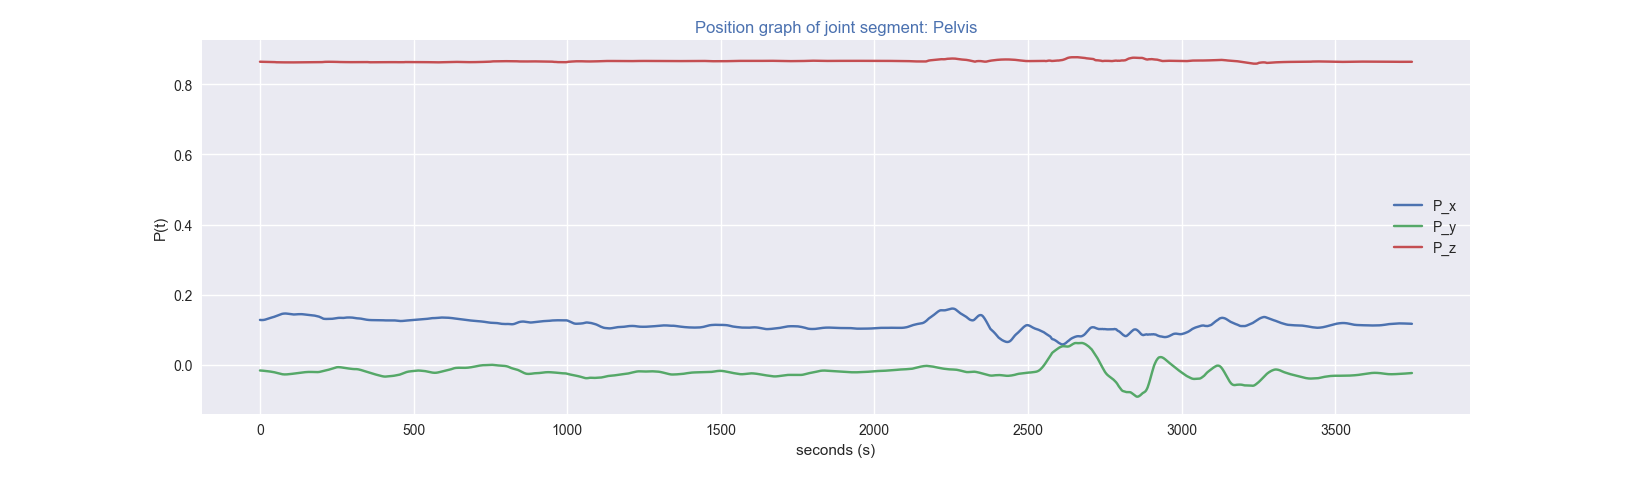
\includegraphics[scale=0.435]{images/xsens-pelvis-position.png}\hfill
    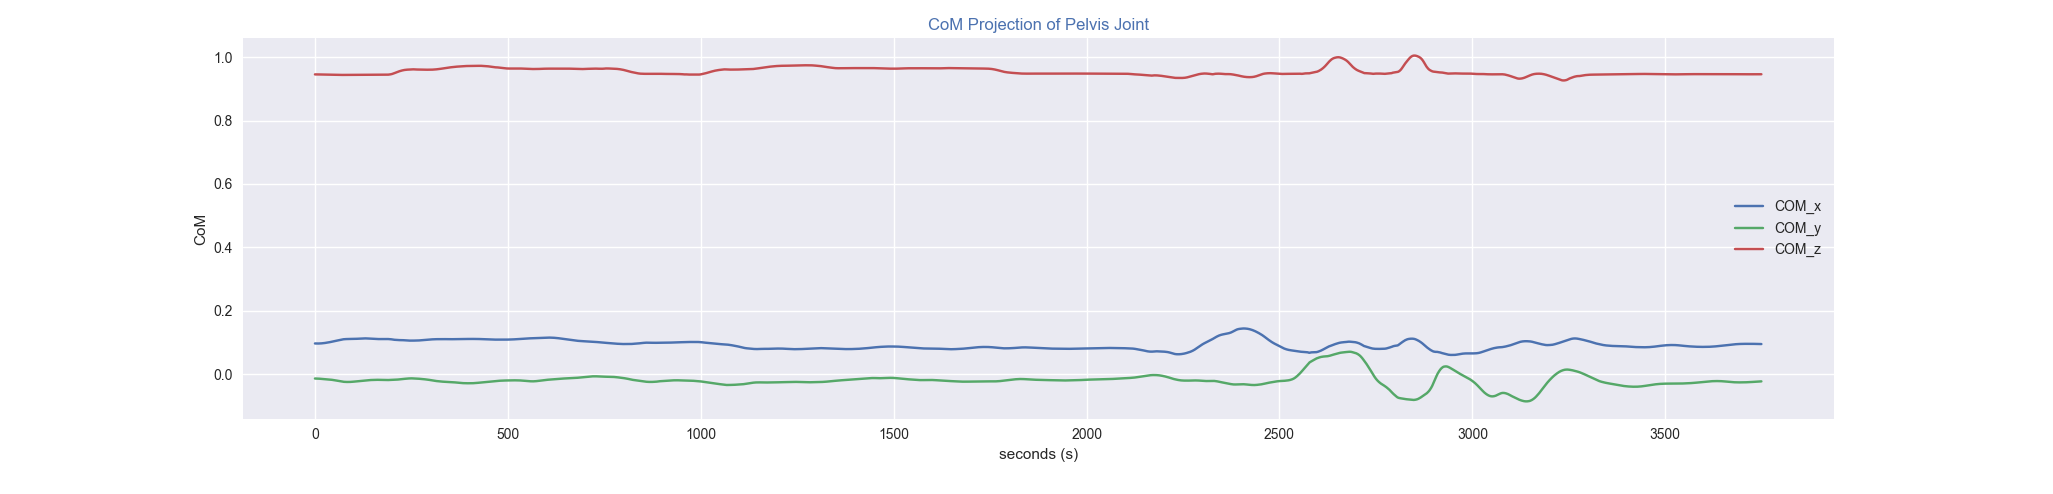
\includegraphics[scale=0.35]{images/xsens-pelvis-com.png}\hfill
    \caption{Xsens data plot pelvis joint}\hfill
    \label{fig: xsens-plot}
\end{figure}

The figure \ref{fig: xsens-plot} represent the position and CoM plot of pelvis joint during the recorded motion. 
The initial stage of the motion is clearly upper body imitation followed by single support and movement along frontal plane of the human actor.